%% $Id: main.tex,v 1.12 2002/08/06 21:23:52 gfu Exp $

\documentclass[fleqn]{article}
%\usepackage[11pt]{times}
\usepackage{graphicx}
\usepackage{amsmath}
\usepackage{url}

\newcommand{\JL}{L^J}
\topmargin -0.5in
\oddsidemargin  0 in
\evensidemargin  0 in
\textwidth   6.5 in
\textheight 9 in

\setlength{\parindent}{0.0in}
\setlength{\parskip}{7pt plus 1pt}
\newcommand{\tight}{\itemsep 0pt}

\newcommand{\code}[1]{{\small \texttt{#1}}}
\newcommand{\email}[1]{{\texttt{#1}}}

\sloppy

\begin{document}

\title{Microsimulation of Urban Development and Location Choices: Design and Implementation of UrbanSim}
\author{P. Waddell $^\dag$ \and A. Borning $^\ddag$ \and M. Noth $^\ddag$ \and N. Freier $^\ddag$ \and M. Becke
$^\ddag$ \and G. F. Ulfarsson $^\circ$
\\\\
$^\dag$ Daniel J. Evans School of Public Affairs and Department of Urban Design and Planning \\ $^\ddag$ Department of Computer Science \& Engineering \\ $^\circ$ Department of Civil and Environmental Engineering \\ University of Washington \\
Seattle, Washington 98195}
\date{}
\maketitle

\subsection*{Abstract}

UrbanSim is a new urban simulation model, developed over the past
several years, which is now operational in three urban areas in
the United States.  The model system is designed to address
emerging needs to better coordinate transportation and land use
planning as a result of recognition of the strong interactions
between land use and transportation, increasing pressure from
federal transportation and environmental legislation, and growing
adoption of state growth management programs. The model system is
implemented as a set of interacting model components that
represent the major actors and choices in the urban system,
including household moving and residential location, business
choices of employment location, and developer choices of locations
and types of real estate development, all subject to the influence
of governmental transportation and land use policy scenarios.  The
model design is unusual in the degree of disaggregation of space,
time, and agents, and in the adoption of a dynamic disequilibrium
approach. The objective of this paper is to describe the entire
system at a sufficient level of detail to convey the key
specification and design choices made in implementing the system.


\section{Introduction}

Transportation models have been in routine use by metropolitan
planning organizations for decades.  However, land use planning is
often not well integrated with transportation planning, despite
their strong interactions. Further, the state of common practice
in land use modeling, and integrated land use and transportation
modeling, is much less advanced than that for transportation
modeling alone.  Some metropolitan regions do no land use modeling
at all.  Others typically use a simple, aggregate model, which is
insensitive to important policy choices regarding zoning, urban
growth boundaries, and taxes and incentives.  The unfortunate
consequence is that the models are then useless for comparing
alternate scenarios involving such policy alternatives.

Considerable progress has recently been made in addressing this
lack.  Over the past several years, we have been designing and
evolving a reusable land use modeling system, named UrbanSim
\cite{noth-architecture-2000,waddell-asce-1998,waddell-env-and-planning-2000},
which has also been integrated with a range of transportation
models. This paper describes version 1.0 of UrbanSim
\cite{urbansim-reference-2000}, released as
Open Source software at {\sf http://www.urbansim.org}. UrbanSim has
evolved from a prototype software system and model application
tested in Eugene-Springfield, Oregon, to a second-generation
production software architecture that has now been used to
implement several versions of the core model components, and has
been subsequently applied in Honolulu, Hawaii and Salt Lake City,
Utah.

% *** somewhere in the paper describe more about what Open Source is
% and what it implies [AB]
% added paragraph near end of introduction [Paul]

UrbanSim differs from other operational urban models in several
prominent characteristics.  The first major design difference is
that it takes a dynamic disequilibrium approach, representing
adjustment processes that occur at different rates, unlike the
cross-sectional equilibrium approach taken in models such as
DRAM/EMPAL \cite{putman-book-1983}, MEPLAN
\cite{echenique-transport-reviews-1990}, or TRANUS
\cite{delabarra-book-1995}. The assumptions underlying equilibrium
models are drawn from general equilibrium in economics, where the
focus is on the analytical insight gained by comparing two steady
state conditions in perfectly competitive markets that differ only
as a result of some exogenous shock to the system.  Equilibrium
analysis in economics is based on assumptions of perfectly
competitive markets, requiring that the actions of any individual
cannot affect prices, the products of all firms in the market are
homogeneous, resources are perfectly mobile (no transaction costs
or delays), and present and future prices and costs are perfectly
known to all market participants.  Moreover, equilibrium requires
that the agendas of all buyers and sellers in all markets be
coordinated simultaneously. When considering the complex
interactions among urban housing, labor and transportation
markets, these assumptions are clearly over-simplifications.

There are at least three different time scales that are relevant
to the interacting system of land use and transportation that
raise serious concern about the appropriateness of full
equilibration. First, travel behavior may change within the scope
of a single day, in response to changes in the transport system.
Let us call this the short-term.  Second, household and business
location choices require somewhat longer to make adjustments to
transport system changes, so that even if we ignore the
transaction costs of moving and the lack of perfect information,
we cannot expect location demand to equilibrate to transport
system changes in the short-term.  Let us call the location choice
adjustment the mid-term.  Third, real estate developers will
respond speculatively to transport system changes and directly to
observed shifts in demand for locations, over yet a longer time
frame of several years that is required by the time to assemble
land and financing, develop plans and obtain permits, extend
infrastructure, and of course, prepare a site and construct
buildings.  We refer to the multiple-year time scale for the real
estate development process as the long-term.

One might suggest that the time scales are irrelevant if we get
the same outcome in the long run, after all the adjustments are
accounted for.  This is unlikely for several reasons. Consider
that during the time frame that a developer is constructing real
estate, processes that occur in the short and mid-term are
changing, so that decisions made at the beginning of the real
estate development process are made sub-optimal by these changes,
resulting in the patterns of over- and under-building so common in
urban real estate markets. Moreover, committed development, even
if misguided and suboptimal, is durable, and influences prices and
availability of real estate opportunities for households and firms
and competing developers, making path-dependence an important part
of the reaction to a transport system change.  And of course, we
know that relocation decisions are constrained by many factors, so
that a change in transportation costs due to a transport system or
pricing change are unlikely to be large enough to cause every
household and business to relocate to an `optimal' location with
respect to balancing transportation and other costs, in the way
that full equilibration requires.

So, if we impose congestion pricing, or open a new highway or rail
system, in year 2010, why should we expect that the real estate
demand and supply would be able to respond in the short-term of
that given year, in the way that a full equilibration of
transportation and land use would suggest?  It might make more
sense to identify the relevant time scales of these three
processes, and assess the degree to which partial equilibration
occurs, as a function of the rate of adjustment of the process.
This is the approach we have taken in the design of
UrbanSim.

Second, the model differs from prior modeling efforts by taking an
extremely disaggregate approach, modeling individual households,
jobs, and real estate development and location choices using grid
cells of $150 \times 150$ meters in size.  The model inputs include
address-level business establishment data, and parcel level land
use and real estate inventories.  The model system microsimulates
the annual evolution in locations of individual households and
jobs, and the evolution of the real estate within each individual
grid cell as the result of actions by real estate developers.  To
our knowledge, no other model system to date has been
operationalized at this level of detail in time, space, and agents.

Third, the model system is implemented within a software
architecture that has been specifically designed to support
disaggregate spatial simulation using a modular approach to the
management of data and model components.  The software is written
in Java, and has been developed as an Open Source project using
the GNU General Public Licence \cite{gpl-web},
which means that anyone can freely
access the source code, modify it, and redistribute it.  The aim
of this approach is simultaneously to encourage collaboration,
improve the openness and transparency of the model system, and
increase the robustness and speed of evolution of the software and
model system.  The Open Source approach to software development,
perhaps the best known example of which is
the Linux operating system, has been increasingly
adopted as a viable and competitive approach, as compared to
proprietary systems.  Our hope is that access to the model without
proprietary restrictions will stimulate rapid innovation in an
area that is in significant need of new approaches, and where
research funds for new development are limited.

These design choices were motivated by the need to address policy
questions that require substantial geographic detail and a level
of behavioral realism inconsistent with general equilibrium
assumptions, within a policy process that is increasingly open to
public scrutiny and participation. Recent reviews of these and
other models can be found elsewhere
\cite{dowling-nchrp-2000,epa-report-2000,miller-tcrp-1999}.  We
review briefly in the next section the software architecture, and
then move to a description of the current model specifications as
applied in Eugene-Springfield. The paper concludes with an
assessment of the current state of the system and plans for its
evolution.


\section{Software Architecture}
\label{sec:overview}

The UrbanSim software architecture has four principal components:

\begin{enumerate}

\item \emph{models} that encode the behavior of agents in the
simulation (such as households and developers), as well as the objects they
operate upon (such as land parcels and buildings),

\item a \emph{model coordinator} that schedules models to run and notifies
them when data of interest has changed,

\item an \emph{object store} that holds the shared representations of agents and other
entities in the simulated world, and

\item a \emph{translation and aggregation layer} that performs a
range of data conversions to mediate between the object store and
the models.

\end{enumerate}

\begin{figure*}
\center \resizebox{0.75
\textwidth}{!}{\includegraphics{arch2.eps}} \caption{UrbanSim
architecture} \label{urbansim-architecture}
\end{figure*}

Models represent different actors or processes in the urban
environment. In addition to encapsulating the behavior of the
actor or process, each model is also responsible for defining the
set of object types it operates on, and the fields of those
objects with which it is concerned.  A model can specify that it
wishes to share fields also declared by other models, thus
providing one technique for data-level coupling and integration of
models via the object store.  A model can also declare new object
types that encapsulate domain-specific data not previously
declared (e.g., a water quality model might declare a nutrient
load value).  A model may specify a set of object types and fields
it wishes to monitor for updates, creations, or deletions.  Each
model is also responsible for indicating how frequently it wishes
to be executed; there are no external constraints on how
frequently or regularly a model need run.

The models do not communicate directly with each other; rather,
they communicate via shared data held in the object store,
mediated by the translation and aggregation layer. This
extensible, modular architecture supports system evolution, in
particular replacing a model with a revised one, and creating and
integrating new models. It allows models to define and share
common sets of objects that they all operate upon, via the object
store (regardless of the original source of the data), and also
allows them to monitor changes to data fields, providing a
convenient method for models to synchronize their actions.
Lastly, it provides the Translation/Aggregation Layer that
automatically performs a range of data conversions that facilitate
model integration.  For example, models can query for zonal
population totals. The Translation/Aggregation Layer computes and
maintains these totals independent of the information in the
object store, which consists of population information at the grid
cell level.

A primary goal of this architecture is to move as much of the
software complexity out of the individual models and into the
supporting infrastructure as possible.  This supporting
infrastructure need be written just once, and can have the
attention of an expert programmer.  The models, on the other hand,
are both numerous and frequently changing.  Often, specifying them
is a complex process, involving considerable domain-specific
knowledge and testing; the more one can relieve the model writers
of programming burdens the better, so that they can concentrate on
issues arising from the domain.


\section{Model Structure}

\begin{figure*}
\center \resizebox{0.7 \textwidth}{!}{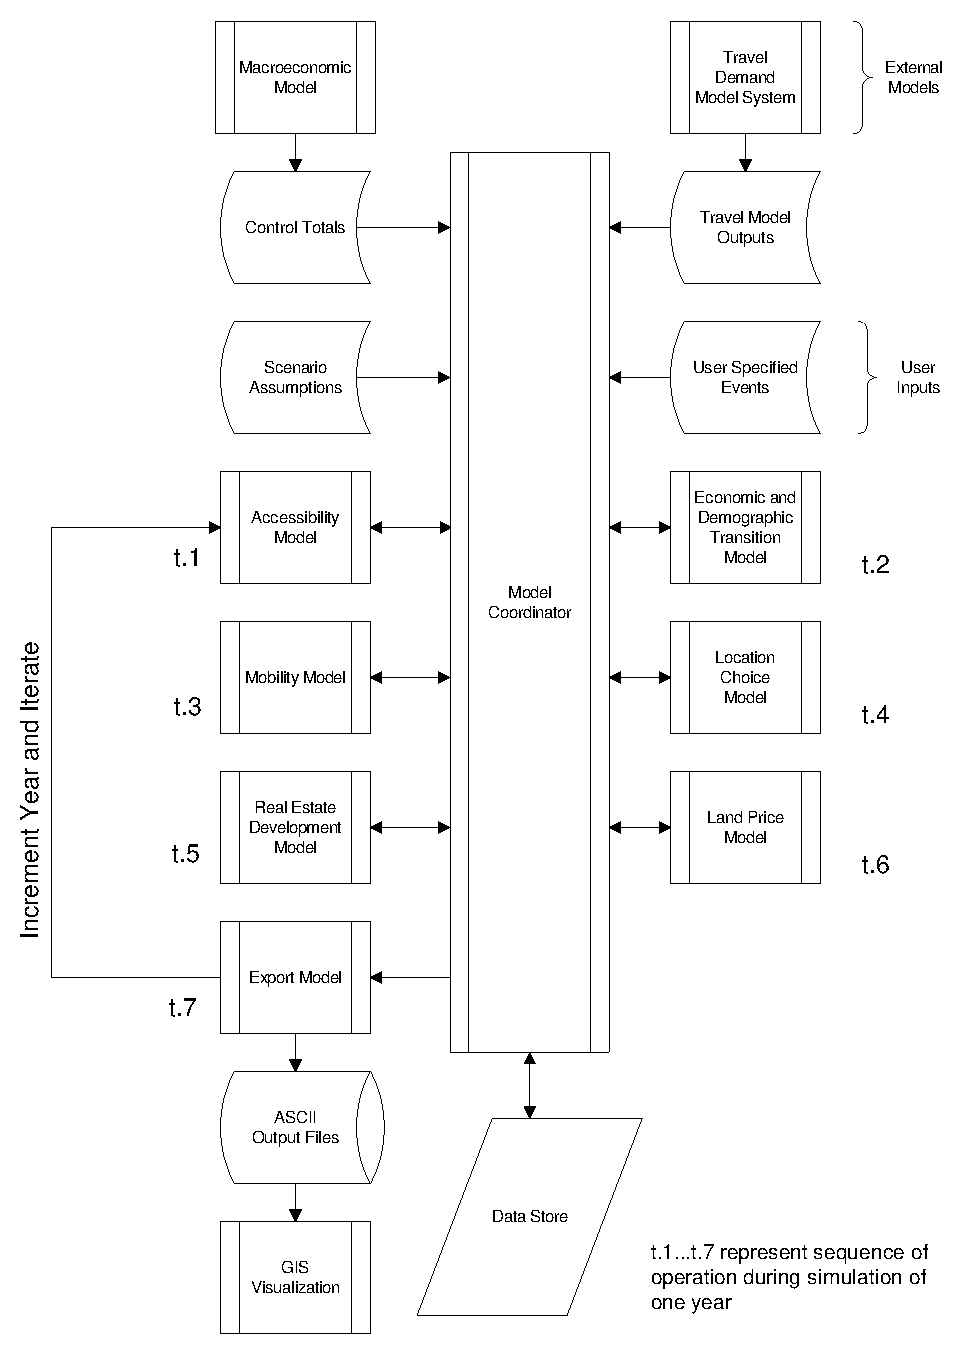
\includegraphics{flow2.eps}}
\caption{UrbanSim Data Flow} \label{urbansim-structure}
\end{figure*}

UrbanSim takes several key inputs as exogenous.  Two of these are
from external model systems: a macroeconomic model to predict
future macroeconomic conditions such as population and employment
by sector, and a travel demand model system to predict travel
conditions such as congested times and composite utilities of
travel between zones.  The latter is loosely coupled to UrbanSim,
with land use predictions input to the external travel models, and
travel conditions input to subsequent annual iterations of the
UrbanSim land use model system.

UrbanSim normally schedules each model to operate once per simulated year,
with the data flow as shown in Figure \ref{urbansim-structure}.  The data
store contains
the current state of all objects in the system, with archiving as
needed by individual models, or as requested by the
user into files for processing by external tools (such
as GIS systems).  Each of the key
models is described in the following subsections.  The
mathematical structure of the underlying procedures in the model
are virtually identical for the household and employment
models, so for brevity the household equations are
omitted from the presentation below.

The system reads exogenous inputs not only from external
macroeconomic and travel demand models, but also from user input.
These user inputs include assumptions reflecting land use policies
that regulate real estate development, and any user-specified
events that describe scheduled events representing changes in
employment, real estate development or land policy the user
intends to apply to the model in a simulation year beyond the
initial or base year.

The main model components, in the order of their execution
in a given simulated year, are
the economic and demographic transition models, the household and
employment mobility models, the accessibility model, the household
and employment location choice models, the real estate development
model, and the land price model.  An output module writes
simulation results in user-specified formats to output files for
further analysis or processing, such as by travel demand models or
by GIS\@.  (For software engineering reasons, the output module is
implemented as a model, namely the Export Model.  Conceptually, however, it
is not a model in the same sense as the others, since it is not an actor or
process in the urban environment, but just reads information and exports it
to external files.)

Locations in the model are based on a grid with a resolution of
$150 \times 150$ meters per grid cell.  Cells are cross-referenced to
Traffic Analysis Zones for indexing travel model outputs, and to
city, county, and other geographic overlays for indexing land use
policies that apply to specific jurisdictions or overlays.

\subsection{Accessibility Model}
\label{accessibility-model}

Since this model is not of the monocentric or spatial interaction
genre, in which the choice of workplace is exogenous and
residential locations are chosen on the basis principally of
commute to the city center or to a predetermined workplace, we
deal with accessibility in a more general framework.  Accessibility
is considered a normal good, like other positive attributes of
housing, on which consumers place a positive economic value.  We
therefore expect that consumers value access to workplaces and
shopping opportunities, among the many other attributes they
consider in their housing preferences. However, not all households
respond to accessibility in the same way. Retired persons would be
less influenced by accessibility to job opportunities than would
working age households, for instance.

% *** regarding ``or alternatively the utility ...'' in the next paragraph:
% is this an alternative, or a different way of saying the same thing?

We operationalize the concept of accessibility for a given
location as the distribution of opportunities weighted by the
composite utility of all modes of travel to those destinations,
defined as the logsum from the mode choice model for each
origin-destination pair. The resulting access measure $A_i$ for
each location $i$ is thus:

\begin{equation}
A_i = \sum_{j=1}^{J} D_j e^{L_{aij}} \end{equation}

\begin{tabbing}

where: \= \hspace*{1cm} \= \\
\> $D_j$ is the quantity of activity in location $j$ \\

\> $L_{aij}$ is the composite utility, or logsum, for households with vehicle
ownership level $a$ \\
\> \> from location $i$ to location $j$ \\
\end{tabbing}

The accessibility model reads the logsum matrix from the travel
model and the land use distribution for a given year, and creates
accessibility indices for use in the household and business
location choice models. The general framework is to summarize the
accessibility from each zone to various activities for which
accessibility is considered important in household or business
location choice.

Since UrbanSim operates annually, but travel model updates are
likely to be executed for only two to three of the years within the
forecasting horizon, travel utilities remain constant from one
travel model run until they are replaced by the next travel model
result. Although travel utilities remain constant between years
for which the travel model system is applied, the activity
distribution in these accessibility indices is updated annually,
so that the accessibility indices change from one year to the next
to reflect the evolving spatial distribution of activities.  There
is considerable disagreement in the literature about how or
whether land use and transportation should be brought to
equilibrium through multiple iterations of the land use and
transportation models.  As discussed in the introduction to the
paper, however, there is little basis for assuming that the
effects of major transportation projects such as rail or highway
systems should instantaneously generate their full effects on land
use.  In reality, land use is likely to respond to transportation
improvements over several years or even decades, depending on the
magnitude of the change.  As a result, we do not propose any
within-year iteration between the land use and transportation
models, and only propose applying the travel models as needed to
reflect system changes, or sufficient land use change to generate
significant differences in congestion patterns.

\subsection{Economic and Demographic Transition Models}
\subsubsection{Economic Transition Model}
\label{economic-transition-model}

Employment is classified by the user into employment sectors based
on aggregations of Standard Industrial Classification codes.
Typically 10 to 20 sectors are defined, based on the local economic
structure. Aggregate forecasts of economic activity and sectoral
employment are exogenous to UrbanSim, and are used as inputs to
the model. These forecasts may be obtained from state economic
forecasts or from commercial or in-house sources.

The Economic Transition Model integrates these exogenous forecasts
of aggregate employment by sector with the UrbanSim database by
computing the sectoral growth or decline from the preceding year,
and either removing jobs from the database in sectors that are
declining, or creating and queuing jobs to be placed in the employment
location choice model for sectors that experience growth.  If the user
supplies only total employment control totals, rather than totals
by sector, the sectoral distribution is assumed consistent with
the current sectoral distribution. In cases of employment loss,
the probability that a job will be removed is assumed proportional
to the spatial distribution of jobs in the sector.  The jobs that
are removed vacate the space they were occupying, and this space
becomes available to the pool of vacant space for other jobs to
occupy in the location component of the model.  This procedure
keeps the accounting of land, structures, and occupants up to
date.

New jobs are not immediately assigned a location.  Instead, new
jobs are added to the database and assigned a null location, to be
resolved by the Employment Location Choice Model
(Section \ref{employment-location-choice-model}).
The model proceeds as follows.

Calculate the number of jobs to be added or removed (a scalar).
Here $|J_{s(t-1)}|$ indicates the number of elements in
(cardinality of) the set $J_{s(t-1)}$.
\begin{equation}
\Delta J_{st} = C_{st} - |J_{s(t-1)}|
\end{equation}
where:
\begin{center}
\begin{tabular}{c p{5.5in}}
$\Delta J_{st}$ & is the change from year $t-1$ to $t$ in total jobs in sector $s$,\\
$C_{st}$ & is the exogenous total employment in sector $s$ in year $t$,\\
%    & $P_{st}$ & is the set of placed jobs in sector $i$ in year $t$, \\
$J_{s(t-1)}$ & is the set of all jobs in sector $s$ in year $t-1$.\\
\end{tabular}
\end{center}

$J_{st}$ is either the union of the previous year's jobs and some newly
created jobs, or the difference between the previous year's jobs and some
number of jobs to remove.

\begin{equation}
J_{st} =
    \begin{cases}
        J_{s(t-1)} \cup F_{st}, &\text{if $\Delta J_{st} > 0$} \\
        J_{s(t-1)},             &\text{if $\Delta J_{st} = 0$}\\
        J_{s(t-1)} - F_{st},    &\text{if $\Delta J_{st} < 0$}
    \end{cases}
\end{equation}
and
\begin{equation}
J_{st} \subset J_{A}
\end{equation}
where:
\begin{center}
\begin{tabular}{c p{5.5in}}
$J_{st}$ & is the set of all jobs in sector $s$ at time $t$, \\
$F_{st}$ & is the set of jobs in flux in sector $s$ in year $t$, \\
$J_{A}$ & is the universe of jobs.\\
\end{tabular}
\end{center}

The jobs in flux are jobs being added or removed from this sector
at this time.  If we are adding jobs, new jobs are taken from the
universe of all jobs and added to the set of jobs present in the
model at time $t$.  If we are removing jobs, the flux jobs are a
random subset of the current jobs of a particular sector in the
model.
\begin{equation}
F_{st} =
    \begin{cases}
        \{\, j \in J_{A} \mid j \notin J_{st},
              j \mbox{ is in sector }s \,\}, &\text{if $\Delta J_{st} > 0$}\\
        \emptyset, &\text{if $\Delta J_{st} = 0$}\\
        \{\, j \in J_{st} \,\}, &\text{if $\Delta J_{st} < 0$}
    \end{cases}
\end{equation}
subject to
\begin{equation}
\label{cardinality-flux-jobs}
| F_{st} | = | \Delta J_{st} |.
\end{equation}
%
(Equation \ref{cardinality-flux-jobs} above constrains the cardinality of
the set of flux jobs to be equal to the absolute value of the change in
number of jobs.)

Let $U_t$ be the set of jobs that do not have a location match at
time $t$. For the base year $t=0$, $U_t$ will initially be the
empty set; in subsequent years it will initially be the remaining
unplaced jobs from the previous year (although typically this will
be the empty set as well).

\begin{equation}
U_t \leftarrow \begin{cases}
        \emptyset & \text{if $t=0$} \\
        U_{t-1}   & \text{otherwise}\\
    \end{cases}
\end{equation}

If we are adding new jobs then they are initially without a
location.  They are added to the set of unplaced jobs and will be
subsequently placed by the Employment Location Choice Model.
\begin{equation}
\text{for each sector $s$: } \;\;
     \text{ if } \Delta J_{st} > 0   \text{ then }
     U_t \leftarrow  U_t \cup F_{st}
\end{equation}

If we are removing jobs then we need to remove the corresponding placed jobs
pairs.
\begin{equation}
\text{for each sector $s$: } \;\;
     \text{ if } \Delta J_{st} < 0   \text{ then }
     P_t \leftarrow P_t - \{\, (j,l) \in P_t \mid j \in F_{st} \,\}
\end{equation}
where:
\begin{center}
\begin{tabular}{c p{5.5in}}
$P_t$ & is the set of all pairs $(j,l)$ representing a job $j$ placed at
location $l$ at time $t$.\\
\end{tabular}
\end{center}

% *** Is there a better way to express this?  The definition of V_t
% seems clunky [Alan}
% V_t used to be U_{lt} but l wasn't really a subscript in the same way
% that t was; it was just to indicate that this was a set of unoccupied
% locations rather than a set of unplaced jobs
% I think the following changes make it less awkward [Paul]

Also, the locations previously occupied by the jobs being removed
must be placed in the set of vacant locations.
\begin{equation}
V_t = \{\, l \in \JL_{t} \mid \forall j \in J_{t} \; (j, l) \notin P_t \,\}
\end{equation}
where:
\begin{center}
\begin{tabular}{c p{5.5in}}
$V_t$ & is the set of locations that do not have a job match at
time $t$,\\
$\JL_{t}$ & is the set of all locations at time $t$ where a job
could be placed,\\
$J_{t}$ & is the set of jobs at time $t$.\\
\end{tabular}
\end{center}


\subsubsection{Demographic Transition Model}

The Demographic Transition Model accounts for changes in the
distribution of households by type over time, using an algorithm
analogous to that used in the Economic Transition Model.  In
reality, these changes result from a complex set of social and
demographic changes that include aging, household formation,
divorce and household dissolution, mortality, birth of children,
migration into and from the region, changes in household size, and
changes in income, among others.  The data (and theory) required
to represent all of these components and their interactions
adequately are not readily available.  Instead, the Demographic
Transition Model, like the Economic Transition Model described
in Section \ref{economic-transition-model},
uses external control totals of population and households
by type (the latter only if available) to provide a mechanism for
the user to approximate the net results of these changes. Analysis
by the user of local demographic trends may inform the
construction of control totals with distributions of household
size, age of head, and income.  If only total population is
provided in the control totals, the model assumes that the
distribution of households by type remains static.

As in the economic transition case, household births are added to
a list of movers that will be located by the Household Location
Choice Model.  Household deaths, on the other hand, are accounted
for in this model by removing those households from the housing
stock, and by properly accounting for the vacancies created by
their departure.  The demographic transition model is analogous in
form to the employment transition model described above.


\subsection{Mobility Models}
\subsubsection{Employment Mobility Model}

Employment mobility and location choices are made by firms.
However, in the current version of UrbanSim, we use individual
jobs as the units of analysis.  This is equivalent to assuming
that businesses are making individual choices about the location
of each job, and are not constrained to moving an entire
establishment.  A prior version of the employment location model
used the business establishment as the unit of analysis.  While
there are advantages to each approach, the main advantage to using
the individual job as the unit of analyis is that it affords greater
capacity for modeling the location of jobs in large businesses.

The Employment Mobility Model predicts the probability that jobs
of each type will move from their current location or stay during
a particular year. This is a transitional change that could
reflect job turnover by employees, layoffs, business relocations,
or closures. Similar to the economic transition model when
handling job losses in declining sectors, the model assumes that
the probability of moving is proportional to the spatial distribution
of jobs in the sector.  All placement of jobs is managed through
the employment location model.

As in the case of job losses predicted in the economic transition
component, the application of this model requires subtracting jobs
by sector from the buildings they currently occupy, and noting
this space as vacant.  These job counts are added to the
unallocated new jobs by sector calculated in the economic
transition model. The combination of new and moving jobs serve as
a pool to be located in the employment location choice model.
Vacancy of nonresidential space is then updated, making space
available for allocation in the employment location choice model.

Since it is possible that the relative attractiveness of
commercial space in other locations when compared with an
establishment's current location may influence its decision to
move, an alternative structure for the mobility model could use
the marginal choice in a nested logit model with a conditional
choice of location. In this way, the model would use information
about the relative utility of alternative locations compared to
the utility of the current location in predicting whether jobs
will move.  While this might be more theoretically appealing than
the specification given, it is generally not supported by the data
available for calibration. Instead, the mobility decision is
treated as an independent choice, and the probabilities estimated
by annual mobility rates directly observed over a recent period
for each sector.  These rates are computed from longitudinally
linked business establishment files, if available.

The resulting form of the employment mobility model is as follows.
$M_{st}$ is a set of jobs that are chosen to be moved based on
$P(j, t)$, a Monte Carlo sampling process using the annual
mobility rate for sector $s$.  This procedure generates a random
number between 0 and 1, and compares it to the cumulative
probability of each possible outcome.  The selected outcome is
then the one that has a cumulative probability interval which
contains the random number.  In the case of only two outcomes,
such as the mobility prediction, the procedure simplifies to an
evaluation of whether the random number is greater than the
mobility probability, in which case the move outcome is chosen.

\begin{equation}
M_{st} = \{\, j \in J_{st} \mid P(j, t) \,\},
\end{equation}
where:
\begin{center}
\begin{tabular}{c p{5.5in}}
$M_{st}$ & is the set of jobs in sector $s$ at time $t$ that are
uprooted by the mobility model,\\
$P(j, t)$ & is a Monte Carlo sampling process determining if job
$j$ will be moved at \mbox{time $t$}.\\
\end{tabular}
\end{center}

The jobs to be moved are now unplaced, and so are added to the unplaced
jobs set:
\begin{equation}
\text{for each sector $s$: } \;\; U_t \leftarrow  U_t \cup M_{st}
%WAS: U_t = U_t \cup M_{st},
\end{equation}
and are removed from the job location pairs set:
\begin{equation}
\text{for each sector $s$: } \;\; P_t \leftarrow  P_t -
    \{\, (j,l) \in P_t \mid j \in M_{st} \,\}.
% WAS: P_t = \{\, (j,l) \in P_t \mid j \notin M_{st} \,\}.
\end{equation}

Finally, the locations previously occupied by the jobs being moved
must be added to the set of vacant locations:
\begin{equation}
V_t = \{\, l \in \JL_{t} \mid \forall j \in J_{t} \; (j, l)
\notin P_t \,\}.
\end{equation}

% *** Again, the definition of V_t seems clunky [Alan}
% better now? [Paul]

\subsubsection{Household Mobility Model}

The Household Mobility Model is similar in form to the Employment
Mobility Model described above.  The same algorithm is used, but
with rates or coefficients applicable to each household type.  For
households, mobility probabilities are estimated from the Census
Current Population Survey, which provides a national database on
which annual mobility rates are computed by type of household.
This will reflect differential mobility rates for renters and
owners, and households at different life stages.

Application of the Household Mobility Model requires subtracting
mover households by type from the housing stock by cell, and
adding them to the pool of new households by type estimated in the
Demographic Transition Model. The combination of new and moving
households serves as a population of households to be located by
the Household Location Choice Model. Housing vacancy is updated as
movers are subtracted, making the housing available for occupation
in the household location and housing type choice model.

\subsection{Location Choice Models}
\subsubsection{Employment Location Choice Model}
\label{employment-location-choice-model}

In this model, we predict the probability that a job that is
either new (from the Economic Transition Model), or has moved
within the region (from the Employment Mobility Model), will be
located at a particular site.  The grid cells used as the basic
geographic unit of analysis in the current model implementation
contain variable quantities of space to be occupied by jobs. The
number of available job locations within a grid cell will depend
mainly on the total square footage of nonresidential floorspace in
the cell, and on the density of the use of space (square feet per
employee). Given the possibility that some jobs will be located in
residential units, however, housing as well as nonresidential
floorspace must be considered in job location.  We have defined a
maximum rate of home-based employment, determined using local data
for a particular metropolitan region, to identify the potential
set of spaces available for home-based employment. The set of job
locations available for placing a job, then, are the union of the
spaces in nonresidential floorspace and a subset of the
residential units in the cell:

\begin{equation}
|L^J_t| = \frac{s_l}{r_{sd}} + \frac{h_l}{r_{hd}}
\end{equation}

% *** define |L^J_t| .

where:
\begin{center}
\begin{tabular}{c p{5.5in}}
$s_l$ & is a scalar representing the total nonresidential square footage of floorspace in location $l$,\\
$h_l$ & is a scalar representing the total number of housing units in location $l$,\\
$r_{sd}$ & is a space utilization rate for nonresidential space
for devtype d (sqft
per employee), \\
$r_{hd}$ & is a home-based employment rate, defined as the minimum
units per job for devtype d
\end{tabular}
\end{center}

For both the employment location and household location models, we
take the stock of available space as fixed in the short run of the
intra-year period of the simulation, and assume that locators are
price takers.  That is, a single locating job or household does
not have enough market power to influence the transaction price,
and must accept the current market price as given.

The variables included in the employment location choice model are
drawn from the literature in urban economics.  We expect that
accessibility to population, particularly high-income population,
increases bids for retail and service businesses.  We also expect
that two forms of agglomeration economies influence location
choices: localization economies and inter-industry linkages.

Localization economies represent positive externalities associated
with locations that have other firms in the same industry nearby.
The basis for the attraction may be some combination of a shared
skilled labor pool, comparison shopping in the case of retail,
co-location at a site with highly desirable characteristics, or
other factors that cause the costs of production to decline as
greater concentration of businesses in the industry occurs.  The
classic example of localization economies is Silicon Valley.
Inter-industry linkages refer to agglomeration economies
associated with location at a site that has greater access to
businesses in strategically related, but different, industries.
Examples include manufacturers locating near concentrations of
suppliers in different industries, or distribution companies
locating where they can readily service retail outlets.

One complication in measuring localization economies and
inter-industry linkages is determining the relevant distance for
agglomeration economies to influence location choices.  At one
level, agglomeration economies are likely to affect business
location choices between states, or between metropolitan areas
within a state.  Within a single metropolitan area, we are
concerned more with agglomeration economies at a scale relevant to
the formation of employment centers.  The influence of proximity
to related employment may be measured using two scales: a regional
scale effect using zone-to-zone accessibilities from the travel
model, or highly localized accessibilities using radial queries of the
area immediately around the given grid cell.  Most of the spatial
queries used in the model are of the latter type, because the
regional accessibility variables tend to be very highly
correlated with each other, and because agglomerations are expected
to be very localized.  (The use of radial queries surrounding grid
cells also avoids the problems of arbitrary zonal aggregations.)

Age of buildings is included in the model to estimate the
influence of age depreciation of commercial buildings, with the
expectation that businesses prefer newer buildings and discount
their bids for older ones.  This reflects the deterioration of
older buildings, changing architecture, and preferences, as is the
case in residential housing.  There is the possibility that
significant renovation will make the actual year built less
relevant, and we would expect that this would dampen the
coefficient for age depreciation.  We do not at this point attempt
to model maintenance and renovation investments and the quality of
buildings.

Density, the inverse of lot size, is included in the location
choice model.  We expect businesses, like households, to reveal
different preferences for land based on their production functions
and the role of amenities such as green space and parking area. As
manufacturing production continues to shift to more horizontal,
land-intensive technology, we expect the discounting for density
to be relatively high.  Retail, with its concentration in shopping
strips and malls, still requires substantial surface land for
parking, and is likely to discount bids less for density.  We
expect service firms to discount for density the least, since in
the traditional urban economics models of bid-rent, service firms
generally outbid other firms for sites with higher accessibility,
land cost, and density.

We might expect that certain sectors, particularly retail, show
some preference for locations near a major highway, and are
willing to bid higher for those locations.  Distance to a highway
is measured in meters, using grid spatial queries.  We also test
for the residual influence of the classic monocentric model,
measured by travel time to the CBD, after controlling for
population access and agglomeration economies.  We expect that,
for most regions, the CBD accessibility influence will be
insignificant or the reverse of that in the traditional
monocentric model, after accounting for the more general measure of
access to employment or population, and other effects.

Calibration of the model is based on a geocoded establishment file
(matched to the parcel file to link employment by type to land use
by type).  The model is estimated using a random sample of
alternative locations, which has been shown to provide consistent
estimates of the coefficients \cite{ben-akiva-lerman-1987}.  A
sample of geocoded jobs in each sector is used to estimate the
coefficients of the location choice model. As with the Household
Location Choice Model, the application of the model produces
demand by each employment type for cell locations.

The employment location model processes each job in the mover
queue in random order, and queries grid cells for alternative
locations to consider. These alternatives are sampled in
proportion to the capacity of the built space in the cell for
accommodating jobs.  The number of alternatives to consider may
be determined by the user.  Jobs may be located in
housing units, as is increasingly the case with home-based
employment through telecommuting and small independent home-based
businesses.  A logit model is applied to estimate the probability
that the current job will move to each of the alternative job
spaces under consideration.  Monte Carlo simulation is used to
generate a decision to locate in a particular alternative, and
once this choice is made, the job is assigned to the cell, and the
respective quantities of vacant and used space in the cell are
updated.  Once a job space been chosen and occupied by a
locating job, it becomes unavailable for consideration by remaining
jobs in the mover queue.

The independent variables used in the employment location choice
model can be grouped into the categories of real estate
characteristics, regional accessibility, and urban-design scale
effects as shown below:

\begin{itemize}

\item Real Estate Characteristics \\
\hspace*{2 mm} \emph{Prices} \\
\hspace*{2 mm} \emph{Development type (land use mix, density)}

\item Regional accessibility \\
\hspace*{2 mm} \emph{Access to population} \\
\hspace*{2 mm} \emph{Travel time to CBD, airport}

\item Urban design-scale \\
\hspace*{2 mm} \emph{Proximity to highway, arterials}

\item Local agglomeration economies within and between sectors: center
formation

\end{itemize}

Using these independent variables, the employment location model
is specified as a multinomial logit model, with separate equations
estimated for each employment sector. The model proceeds as
follows.

The job location pairs set contains all pairs of placed jobs
and their locations.

\begin{align}
P_t &= \{\, (j, l) \mid j \in J_{t}, l \in \JL_{t}, \text{job $j$
  is placed at location $l$} \,\},\\
U_t &= \{\, j \mid j \in J_{t}, \forall l \in \JL_{t} \;
     (j, l) \notin P_t \,\},\\
V_t &= \{\, l \mid l \in \JL_{t}, \forall j \in J_{t} \;
     (j, l) \notin P_t \,\},\\
D_{st} &= \{\, (l, p) \mid l \in V_t, \text{ $p$ is the
   probability of a job in sector $s$ locating in $l$} \,\}
\end{align}
where:
\begin{center}
\begin{tabular}{c p{5.5in}}
$D_{st}$ & is the set of pairs representing the probability of an
employee of sector $s$ locating to a particular location at time $t$.\\
\end{tabular}
\end{center}

Monte Carlo sampling of the location choices for each sector
occurs over the distribution given by $D_{st}$.
\begin{align}
F_t = \{\, (j, l) \mid j \in U_t, &\text{ Monte Carlo
choice of $l$ from $D_{st}$ given the sector of $j$} \,\},
\end{align}
where:
\begin{center}
\begin{tabular}{c p{5.5in}}
$F_t$ & is the set of new job/location pairs created using a
Monte Carlo sampling from $D_{st}$ for each sector.\\
\end{tabular}
\end{center}

The cardinality of the set of new job/location pairs is constrained to be
equal to the cardinality of the set of unplaced jobs or of the set of
unoccupied locations, whichever is smaller.
\begin{equation}
|F_t| = \min( |U_t|, |V_t| ).
\end{equation}

Finally, the set of job/location pairs is modified to reflect the
new matchings, the placed jobs are removed from the set of
unplaced jobs, and the newly occupied locations are removed from
the set of vacant locations.
\begin{align}
P_t & \leftarrow P_t \cup F_t \\
U_t & \leftarrow U_t - \{\, j \in U_{t} \mid \exists l \, (j,l) \in F_t \,\} \\
V_t & \leftarrow V_t - \{\, l \in V_{t} \mid \exists j \, (j,l) \in F_t \,\}
\end{align}

% *** Paul: please check the above equations.  If these seem reasonable,
% maybe the V_t equations (marked 'clunky' previously) could be rewritten
% in this form.

\subsubsection{Household Location Choice Model}

In this model, as in the employment location model, we predict the
probability that a household that is either new (from the
transition component), or has decided to move within the region
(from the mobility component), will choose a particular location
defined by a grid cell.  As before, the form of the model is
specified as multinomial logit, with random sampling of
alternatives from the universe of available (vacant) housing
units, including those units vacated by other movers in the current
year.

The model architecture allows location choice models to be
estimated for households stratified by income level, the presence
or absence of children, and other life cycle characteristics.
Alternatively, these effects can be included in a single model
estimation through interactions of the household characteristics
with the characteristics of the alternative locations.  The
current implementation is based on the latter, but is general
enough to accommodate stratified estimation, for example by
household income. The variables used in the model are drawn from
the literature in urban economics, urban geography, and urban
sociology.  An initial feature of the model specification is the
incorporation of the classical urban economic trade-off between
transportation and land cost. This has been generalized to account
not only for travel time to the classical monocentric center, the
CBD, but also to more generalized access to employment
opportunities and to shopping. These accessibilities to work and
shopping are measured by weighting the opportunities at each
destination zone with a composite utility of travel across all
modes to the destination, based on the logsum from the mode choice
travel model.

These measures of accessibility should negate the traditional pull
of the CBD, and, for some population segments, potentially reverse
it.  In addition to these accessibility variables, we include in
the model a net building density, to measure the
input-substitution effect of land and capital.  To the extent that
land near high accessibility locations is bid up in price, we
should expect that builders will substitute capital for land and
build at higher densities.  Consumers for whom land is a more
important amenity will choose larger lot housing with less
accessibility, and the converse should hold for households that
value accessibility more than land, such as higher income
childless households.

The age of housing is considered for two reasons.  First, we
should expect that housing depreciates with age, since the
expected life of a building is finite, and a consistent stream of
maintenance investments are required to slow the deterioration of
the structure once it is built.  Second, due to changing
architectural styles, amenities, and tastes, we should expect that
the wealthiest households prefer newer housing, all else being
equal.  The exception to this pattern is likely to be older,
architecturally interesting, high quality housing in historically
wealthy neighborhoods.  The preference for these alternatives are
accommodated through a combination of nonlinear or dummy variable
treatment for this type of housing and neighborhood.

A related hypothesis from urban economics is that, since housing
is considered a normal good, it has a positive income elasticity
of demand.  This implies that as incomes rise, households will
spend a portion of the gains in income to purchase housing that is
more expensive, and that provides more amenities (structural and
neighborhood) than their prior dwellings.  A similar hypothesis is
articulated in urban sociology in which upward social mobility is
associated with spatial proximity to higher status households.
Both of these hypotheses predict that households of any given
income level prefer, all else being equal, to locate in
neighborhoods that have higher average incomes.  (UrbanSim does
not attempt to operationalize the concepts of social status or
social assimilation, but does consider income in the location
choice.)

The age hypothesis and the two income-related hypotheses are
consistent with the housing filtering model, which explains the
dynamic of new housing construction for wealthy households that
sets in motion a chain of vacancies.   The vacancy chain causes
households to move into higher status neighborhoods than the ones
they leave, and housing units to be successively occupied by lower
and lower status occupants.  At the end of the vacancy chain, in
the least desirable housing stock and the least desirable
neighborhoods, there can be insufficient demand to sustain the
housing stock and vacancies go unsatisfied, leading ultimately to
housing abandonment.  We include in the model an age depreciation
variable, along with a neighborhood income composition set of
variables, to collectively test the housing filtering and related
hypotheses.

Housing type is included in the model as a set of dummy variables
for alternative development types.  Development types correspond
to the density and land use mix within a cell, with multiple
categories of residential development, and mixed use development
encompassing both commercial space and residential housing.  These
are discussed further in Section
\ref{real-estate-development-model} describing the real estate
development model.

One of the features that households prefer is a compatible land
use mix within the neighborhood.  It is likely that residential
land use, as a proxy for land uses that are compatible with
residential use, positively influences housing bids.   On the
other hand, industrial land use, as a proxy for less desirable
land use characteristics, would lower bids.  There is some
evidence that mixed use neighborhoods that contain retail and
services, in the form advocated by proponents of new urbanist or
neotraditional neighborhood design, are positively valued.  We
test this using the proximity of retail employment within walking
distance.

% *** how does this relate to neo-traditional/New Urbanist theories, which
% say that mixed use (residential/retail) is desirable?
% good point, see 2 new sentences added above [Paul]

The household location model is estimated using a random sampling
of alternative locations, as is the case in the employment
location model. In application, each locating household is modeled
individually, and a sample of alternative cell locations is
generated in proportion to the available (vacant) housing. Monte
Carlo simulation is used to select the specific alternative to be
assigned to the household, and vacant and occupied housing units
are updated in the cell.

% *** is the description in the following paragraph describe one of the
% existing real systems, or is it a straw man?
% it is a flowery interpretation of what we've actually implemented [Paul]

The market allocation mechanism used to assign households and jobs
to available space, then, is not done through a general
equilibrium solution in which consumers and suppliers optimize
across all alternatives based on perfect information, and zero
transaction costs, with prices on all buildings at each location
adjusting to the general equilibrium solution that perfectly
matches consumers and suppliers to clear the market. Rather, the
solution is based on an expectation of incomplete information (we
sample alternatives) and nontrivial transaction and search costs
(only a fraction of jobs and households move annually), so that
movers attempt to obtain the most satisfactory location from the
sampled vacant real estate stock.  Prices respond at the end of
the year to the characteristics of locations and the balance of
demand and supply (vacancy rates) at each location.

% *** should this be ``obtain the most desirable location among those known
% to be available'' or something like that?
% see change above [Paul]

The independent variables can be organized into the three
categories of housing characteristics, regional accessibility, and
urban-design scale effects as shown below.

\begin{itemize}

\item{Housing Characteristics} \\
\hspace*{2 mm} \emph{Prices (interacted with income) \\
\hspace*{2 mm} Development types (density, land use mix) \\
\hspace*{2 mm} Housing age}

\item{Regional accessibility} \\
\hspace*{2 mm} \emph{Job accessibility by auto-ownership group \\
\hspace*{2 mm} Travel time to CBD and airport}

\item{Urban design-scale (local accessibility)} \\
\hspace*{2 mm} \emph{Neighborhood land use mix and density \\
\hspace*{2 mm} Neighborhood employment}

\end{itemize}

\subsection{Real Estate Development Model}
\label{real-estate-development-model}

\subsubsection{Data}
The real estate developer model simulates the construction of new
real estate, either through the construction of new development or
the intensification or conversion of existing development.  The
data is structured as grid cells, currently specified as
$150 \times 150$ meters in resolution (though this is a specification issue
and not a restriction in the software). Parcel data is
preprocessed to obtain the intersection of parcels and grid cells,
and then to construct a composite representation of the real
estate development within each cell.  Cells are then classified on
the basis of their real estate composition, into `Development
Types', as shown in Table~\ref{development-types}.  The classification
is based on the number of housing units in a cell, and the quantity of
nonresidential square footage in the cell.  Cells containing some
housing and almost no nonresidential square footage are considered
residential in character.  Those containing a diverse mixture of housing
and nonresidential floorspace are considered mixed-use, and those cells
containing principally nonresidential square footage are further classified
into commercial, industrial or governmental types.

The data to estimate the coefficients for the developer model is
derived from preprocessing the parcel and grid data, making heavy
use of the year built values of the existing development in the
assessor records.  The data preparation procedure imputes year
built values for those records for which it is missing by examining the
surrounding cells of the same type and drawing from the
distribution of observed values.  Once the data is complete,
historical development `events' are identified for some
user-specified period of time, and these events are extracted to a
file for further analysis.  Events, within this framework, are any
changes in the real estate development within a cell that is
identified by examining the year built values within the data.
This means that the procedure is capable of identifying any new
construction that has a year built occurring within the specified
time frame.  However, it does not identify events that involve
the demolition of buildings at some time in the past,
since normally there is no record of such demolished buildings
within the current assessor database.  This procedure
could be augmented with data derived from building demolition and
permit records, but that has not been accounted for in the current
specification.

The result of this procedure, then, is the production of a set of
development events that represent all observed transitions between
any pairs of development types within each year of the specified
historical time frame.  The time slice for determining
the existence of an event is annual, since this is the limit of
the information on the vintage of real estate.  Also, some
development events may be observed in the data that do not indicate a
change of development type, but rather an intensification of use
within the range specified in the definition of the development
types.

\begin{table}[t]
\begin{center}
\begin{tabular}{llccl}
DevType & Name & Units &  Sqft  &  Primary Use  \\ \hline
1 &  R1 & 1       & $< 1,000$ & Residential \\
2 &  R2 & 2 - 4   & $< 1,000$ & Residential \\
3 &  R3 & 5 - 9   & $< 1,000$ & Residential \\
4 &  R4 & 10 - 14 & $< 2,500$ & Residential \\
5 &  R5 & 15 - 21 & $< 2,500$ & Residential \\
6 &  R6 & 22 - 30 & $< 2,500$ & Residential \\
7 &  R7 & 31 - 75 & $< 5,000$ & Residential \\
8 &  R8 & $\geq 76$ & $< 5,000$ & Residential \\
9 &  M1 & 0 - 9   & 1,000 - 4,999 & Mixed R/C \\
10 & M2 & 10 - 30 & 2,500 - 4,999 & Mixed R/C \\
11 & M3 & 10 - 30 & 5,000 - 24,999 & Mixed R/C \\
12 & M4 & 10 - 30 & 25,000 - 49,999 & Mixed R/C \\
13 & M5 & 10 - 30 & $\geq 50,000$ & Mixed R/C \\
14 & M6 & $\geq 31$ & 5,000 - 24,999 & Mixed R/C \\
15 & M7 & $\geq 31$ & 25,000 - 49,999 & Mixed R/C \\
16 & M8 & $\geq 31$ & $\geq 50,000$ & Mixed R/C \\
17 & C1 & $< 10$ & 1,000 - 24,999 & Commercial \\
18 & C2 & $< 10$ & 25,000 - 49,999 & Commercial \\
19 & C3 & $< 10$ & $\geq 50,000$ & Commercial \\
20 & I1 & $< 10$ & 1,000 - 24,999 & Industrial \\
21 & I2 & $< 10$ & 25,000 - 49,999 & Industrial \\
22 & I3 & $< 10$ & $\geq 50,000$ & Industrial \\
23 & GV & $\geq 0$ & $\geq 0$ & Government \\
24 & VC & 0 & 0 & Vacant Dev \\
25 & UN & 0 & 0 & Undevelopable
\end{tabular}
\caption{Development Types}
\label{development-types}
\end{center}
\end{table}

\subsubsection{Structure}

The developer model is structured to predict the probability
within a single simulation year of a grid cell experiencing a
development event, and if it does experience such an event,
identifying the type of event that is most likely. A multinomial
logit model is used to estimate these probabilities. Once these
probabilities are estimated for a grid cell, commitment of
development is simulated using a Monte Carlo sampling process.
Implementation of the development takes place by using a
development template to obtain the most likely characteristics of
the resulting development project within the cell, including the
number of housing units, square feet of commercial, industrial and
government space, improvement value, and construction schedule.
These commitments are then added to the `development event' queue,
to be built (added to the database) as scheduled.

Constraints on development outcomes are included through a
combination of user-specified spatial overlays and decision rules
about specific types of development allowed in different
situations.  Each cell is assigned a series of overlays through
spatial preprocessing using GIS overlay techniques. These overlays
can be used to assign user-specified constraints on the type of
development that is allowed to occur within each of these overlay
designations.  The constraints are indicated as allowed
conversions between each land use plan designation and each
development type in a file supplied by the user as part of the
construction of a scenario for simulation. Those conversions that
are contained in this file are not considered in the model. This
is implemented by eliminating them from the choice set for any
cell affected by the constraint. These constraints are therefore
interpreted as binding constraints, and not subject to market
pressure.  Currently, if users wish to examine the impact of these
constraints, they would need to relax a particular constraint
within one scenario and compare the scenario results to a more
restrictive policy.  The overlays used in the Eugene-Springfield
model application include the following features:

\begin{itemize}
\tight
\item  Land use plan designation
\item  City
\item  County
\item  Wetland designation
\item  Floodplain/floodway
\item  Stream or riparian buffer
\item  High slope areas
\item  Urban Growth Boundary
\end{itemize}


The independent variables used in the real estate development
model can be organized into categories of site characteristics,
urban design-scale effects, regional accessibility, and market
conditions, as shown below:

\begin{itemize}
\item Site characteristics \\
\hspace*{2 mm} \emph{Existing development characteristics \\
\hspace*{2 mm} Land use plan \\
\hspace*{2 mm} Environmental constraints}

\item Urban design-scale \\
\hspace*{2 mm} \emph{Proximity to highway and arterials \\
\hspace*{2 mm} Proximity to existing development \\
\hspace*{2 mm} Neighborhood land use mix and property values \\
\hspace*{2 mm} Recent development in neighborhood}

\item Regional accessibility \\
\hspace*{2 mm} \emph{Access to population and employment \\
\hspace*{2 mm} Travel time to CBD, airport}

\item Market Conditions \\
\hspace*{2 mm} \emph{Vacancy rates}
\end{itemize}

% *** Need more overview here.  where is the result from running the model,
% for instance? [Alan]

Using these variables, the real estate development model simulates
the probability of each possible transition from one development
type to another, for every cell in the model database. The model
proceeds as follows.

\begin{align}
T &= \{\, (d_1, d_2) \mid \text{devtype $d_1$ can transition to devtype $d_2$} \,\},\\
T_{lt} &= \{\, d_2 \mid (d_1, d_2) \in T, l \in L_{t}, \text{$d_1$
is the
devtype of $l$} \,\},\\
P_{lt} &= \{\, (d, p) \mid j \in T_{tl}, \text{ $p$ is the
probability of transitioning to devtype $d$ at location $l$} \,\},
\end{align}
where:
\begin{center}
\begin{tabular}{c p{5.5in}}
$T$ & is the set of valid development type transitions,\\
$T_{lt}$ & is the set of all valid development type transitions at location $l$ at time $t$,\\
$L_{t}$ & is the set of all locations at time $t$,\\
$P_{lt}$ & is the set of probabilities of transitioning to a
particular development type at location $l$ at time $t$.\\
\end{tabular}
\end{center}

The development type for each location is defined to be the outcome of the
chosen transition.  One probable transition is one that includes
no change.

We can then define the set $L_{dt}$ of location and development type pairs
at time $t$ as follows:
\begin{equation}
L_{dt} = \{\, (l, d) \mid (d, p) \in P_{lt}, l \in L_{t}, \text{
$d$ is chosen given a Monte Carlo sampling of $p$} \,\}
\end{equation}

\subsection{Land Price Model}

UrbanSim uses land prices as the indicator of the match between
demand and supply of land at different locations and with
different development types, and of the relative market valuations
for attributes of housing, nonresidential space, and location.
This role is important to the rationing of land and buildings to
consumers based on preferences and ability to pay, as a reflection
of the operation of actual real estate markets. Since prices enter
the location choice utility functions for jobs and households, an
adjustment in prices will alter location preferences.  All else
being equal, this will in turn cause higher price alternatives to
become more likely to be chosen by occupants who have lower price
elasticity of demand.  Similarly, any adjustment in land prices
alters the preferences of developers to build new construction of various
types and densities.

We make the following assumptions:

\begin{enumerate}

\item Households, businesses, and developers are all
price-takers, and market adjustments are made by the market in
response to aggregate demand and supply relationships.  Each
responds, therefore, to previous period price information.

\item
Location preferences and demand-supply imbalances are capitalized
into land values.  Building value reflects building replacement
costs only, and can include variations in development costs due to
terrain, environmental constraints, or development policy.

\item
There is a long-term structural vacancy rate for each type of
property, and the relationship of current vacancy rates to this
long-term vacancy rate influences price adjustments.
\end{enumerate}

Land prices are modeled using a hedonic regression
\cite{waddell-hedonic-1993} of land value on attributes of the
land and its environment, including land use mix, density of
development, proximity of highways and other infrastructure, land
use plan or zoning constraints, and neighborhood effects.  The
hedonic regression may be estimated from sales transactions if
there are sufficient transactions on all property types, and if
there is sufficient information on the lot and its location.  An
alternative is to use tax assessor records on land values, which
are part of the database typically assembled to implement the
model.  Although assessor records may contain biases in their
assessment, they do provide virtually complete coverage of the
land (with notable exceptions and gaps for exempt or publicly
owned property).

The hedonic regression equation encapsulates interactions between
market demand and supply, revealing an envelope of implicit
valuations for location and structural characteristics.  These
relative prices have been documented to be relatively consistent
over time, with the acknowledgment that the relative values at
specific locations change as their underlying characteristics
change \cite{dipasquale-wheaton-1996}.  Because the hedonic
regression includes variables that are to be maintained as part of
the simulation system, these can be used to update relative prices
over time.

In addition to these relative prices captured by the hedonic
regression, the overall price level within the market for each
type of real estate moves over time in response to shifts between
supply and demand.  These fluctuations can be tied to the
relationship between the actual market vacancy rate and the
long-term structural vacancy rate.  When the current vacancy rate
falls below the structural rate, price levels rise, and when the
current vacancy rate exceeds the structural level, they fall.

These two effects on prices are combined in the land price model.
The estimated hedonic regression equation is used to establish
relative prices, and the intercept of the equation is adjusted
based on the relative position of the current and structural
vacancy rate, as follows:

\begin{equation} P_{ilt} =\alpha +
\delta \left(\frac{V^s_i - V^c_{it}}{V^s_{i}}\right) +
\beta X_{ilt}
\end{equation}

\begin{tabbing}
where: \= \\
    \> $P_{ilt}$ is the price of land per acre of development type $i$
    at location $l$ at time $t$ \\
    \> $V^c_{it}$ is the current vacancy rate at time $t$, weighting
    local and regional vacancy \\
    \> $V^s_i$ is the long-term structural vacancy rate \\
    \> $X_{ilt}$ is a vector of locational and site attributes \\
    \> $\alpha$, $\delta$ and $\beta$ are estimated parameters
\end{tabbing}

Prices are updated annually, after all construction and market
activity is completed.  These end-of-year prices are then used as
the values of reference for market activities in the subsequent
year.

The independent variables influencing land prices can be organized
into site characteristics, regional accessibility, urban-design
scale effects, and market conditions, as shown below:

\begin{itemize}

\item Site characteristics \\
\hspace*{2 mm} \emph{Development type \\
\hspace*{2 mm} Land use plan \\
\hspace*{2 mm} Environmental constraints}

\item Regional accessibility \\
\hspace*{2 mm} \emph{Access to population and employment}

\item Urban design-scale \\
\hspace*{2 mm} \emph{Land use mix and density \\
\hspace*{2 mm} Proximity to highway and arterials}

\item Market Conditions \\
\hspace*{2 mm} \emph{Vacancy rates}

\end{itemize}

\subsection{User-Specified Events}

Given our current understanding, no model will be able to simulate
accurately the timing, location and nature of major events such as
a major corporate relocation into or out of a metropolitan area,
or a major development project such as a regional shopping mall.
In addition, major policy events, such as a change in the land use
plan or in an Urban Growth Boundary, are outside the range of
predictions of our simulation.  (At least in its current form,
UrbanSim is intended as a tool to aid planning and civic
deliberation, not as a tool to model the behavior of voters or
governments.  We want it to be used to say ``if you adopt the
following policy, here are the likely consequences," but not to
say ``UrbanSim predicts that in 5 years the county will adopt the
following policy.")

However, planners and decision-makers often have information about
precisely these kinds of major events, and there is a need to
integrate such information into the use of the model system.  It
is useful, for example, to explore the potential effects of a
planned corporate relocation by introducing user-specified events
to reflect the construction of the corporate building, and the
relocation into the region (and to the specific site) of a
substantial number of jobs, and examine the cumulative or
secondary effects of the relocation on further residential and
employment location and real estate development choices.  Inability
to represent such events, in the presence of knowledge about
developments that may be `in the pipeline,' amounts to less than
full use of the available information about the future, and could
undermine the validity and credibility of the planning process.
For these reasons, support for three kinds of events has been
incorporated into the system: development events, employment
events, and policy events.

The software architecture implements simulated events generated by
the model components, each of which are time-stamped to occur at a
specified time in the future.  The user-specified events leverages
this facility of the model coordinator within the software
architecture, to scan for user specified events in a series of
input files prepared by the user.  The user defines events
according to a specified format, indicating the cells affected,
the date at which the event should occur, and the other relevant
attributes of the development, employment, or policy event.  The
model coordinator implement these events at the beginning of the
specified year, prior to generating simulated events in the model
components.

% *** More needed here.  How is support for the different kinds of events
% incorporated?  How are they input?
% added above paragraph.  Could do more but this may suffice [Paul]

\section{Conclusion}
This paper provides a detailed  description of the implementation
of version 1.0 of UrbanSim, a land use model system designed to
integrate with travel demand models in support of metropolitan
land use and transportation planning and growth management.  The
model system is operational and has been applied in three
metropolitan areas in the U.S. When released on the Internet as
Open Source software in the second quarter of 2000, it was
downloaded over 300 times in countries spread over five
continents.  The model system is undergoing continuous
development, and is available at {\sf http://www.urbansim.org}.

Short term (current year) development of the model system is
focusing on:

\begin{itemize}
\item Developing a graphical user interface for the model,\
\item Develping visualization tools for comparing scenario results,\
\item Developing a software system for data integration and synthesis for applying the model system in other locales using
available data,\
\item Developing a design for an extended model system that integrates household choices of
activity and travel pattern, vehicle ownership, job location and
residential location, essentially dissolving the artificial
distinction between land use and travel demand models.\
\end{itemize}

The longer-term research agenda includes:
\begin{itemize}
\item Further developing the software architecture
to support multi-agent microsimulation efficiently, and developing
a high level model specification language;\
\item Exploring new model structures and estimation techniques,
such as Bayesian networks \cite{jensen-bayesian-1996}, that may provide
greater flexibility in representing the complex choice behavior
and interdependence than has been feasible in either random
utility maximization or decision heuristic approaches to date;\
\item Developing new model components representing environmental
processes and impacts, including land cover change, water demand,
and nutrient emissions.
\end{itemize}

The UrbanSim project represents a long-term collaborative research
agenda to improve the state of the practice in metropolitan land
use and transportation planning and growth management, and the
results reported here document a significant milestone in this
agenda.

\subsection*{Acknowledgments}

Many people have contributed to UrbanSim.  Thanks in particular to
A.J. Bernheim Brush, David Chang, Matthew Dockrey, Leo Lai, Dorian Miller,
and Denise Pinnel for work on the software, and to Kevin Krizek, John
Carruthers and Robert Willis for work on data analysis and model
calibration.  This research has been funded in part by National Science
Foundation Grant No.~CMS-9818378, and in part by the University of
Washington PRISM project.


\newpage

\bibliography{urbansim}
\bibliographystyle{plain}

\end{document}

% LocalWords:   Exp UrbanSim Waddell Noth Freier Becke Ulfarsson EMPAL MEPLAN
% LocalWords:  TRANUS USDiag eps macroeconomic GIS logit Carlo DevType GV
% LocalWords:  preprocessed Sqft VC Floodplain arterials CBD devtype sqft
% LocalWords:  transitioning floorspace co accessibilities agglomerations
% LocalWords:  geocoded telecommuting jt logsum downloaded Bernheim Dockrey CMS
% LocalWords:  Denise Krizek Carruthers Willis
